%% LaTeX-Beamer template for KIT design
%% by Erik Burger, Christian Hammer
%% title picture by Klaus Krogmann
%%
%% version 2.1
%%
%% mostly compatible to KIT corporate design v2.0
%% http://intranet.kit.edu/gestaltungsrichtlinien.php
%%
%% Problems, bugs and comments to
%% burger@kit.edu

\documentclass[18pt]{beamer}

%% SLIDE FORMAT

% use 'beamerthemekit' for standard 4:3 ratio
% for widescreen slides (16:9), use 'beamerthemekitwide'

\usepackage{templates/beamerthemekit}
\usepackage[utf8]{inputenc}
% \usepackage{templates/beamerthemekitwide}

%% TikZ INTEGRATION

% use these packages for PCM symbols and UML classes
\usepackage{templates/tikzkit}
% \usepackage{templates/tikzuml}
\usepackage{listings}
\usepackage{tabulary}

\selectlanguage{ngerman}

\title[Treppenerkennung für einen treppensteigenden Roboter]{Treppenerkennung für einen treppensteigenden Roboter}
\subtitle{Projektpraktikum Robotik und Automation I (Software)}
\author{Maximilian Heß}

\institute{Institut für Anthropomatik und Robotik (IAR) - Intelligente Prozessautomation und Robotik (IPR)}

% Bibliography

\usepackage[citestyle=authoryear,bibstyle=numeric,hyperref,backend=biber]{biblatex}
\addbibresource{templates/example.bib}
\bibhang1em

\begin{document}

%title page
\begin{frame}
	\titlepage
\end{frame}

%table of contents
\begin{frame}{Übersicht}
	\tableofcontents
\end{frame}



\section{Motivation}

\begin{frame}{Motivation}
	\begin{itemize}
		\item Ziel: Finden und Kartografieren von Treppen
		\item Ermöglicht die Einführung von Ebenen in 2D-Karten
		\item Verknüpfung der Ebenen mittels Treppenmarkierungen
		\item Anwendungsbeispiel: Wegfindung über mehrere Stockwerke
	\end{itemize}
\end{frame}



\section{Hintergrund}

\subsection{Roboterplattform - HMMWV}
\begin{frame}{Roboterplattform - HMMWV}
	\begin{itemize}
		\item Hardwareausstattung Basisversion
		\begin{itemize}
			\item Sick LMS 100 (LiDAR) zum 2-dimensionalen Mappen und Lokalisieren
			\item Brix mit Intel Core 2Duo..
			\item ATmega-basiertes Steuerinterface (Atmel ATmega 2560)
			\item WLAN-Router
		\end{itemize}
		\item Hardwareerweiterungen für die Treppenerkennung
		\begin{itemize}
			\item Schnellerer Brix für 3D-Berechnungen
			\item Asus Action Camera für 3D-Erfassung der Umgebung
		\end{itemize}
	\end{itemize}
\end{frame}

\begin{frame}{Roboterplattform - HMMWV}
	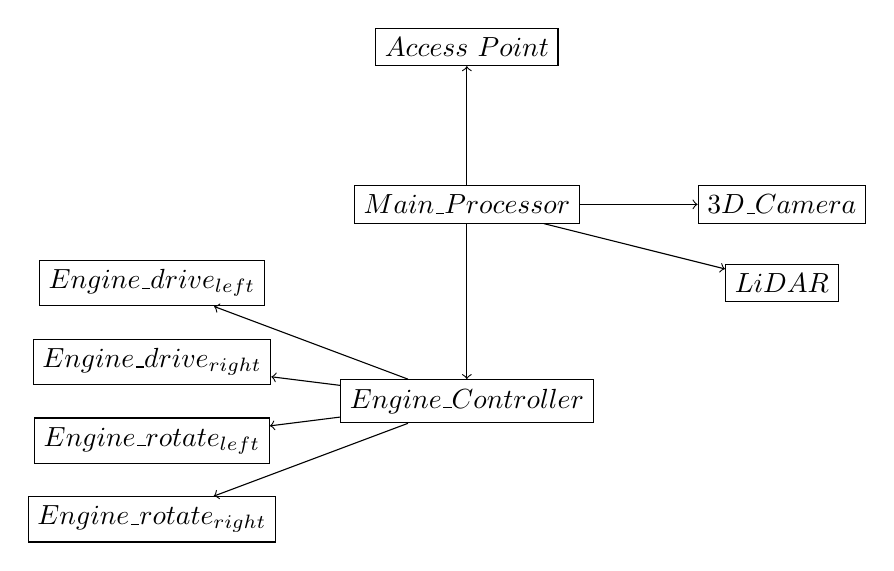
\begin{tikzpicture}
		\node at (0,   3) [rectangle,draw] (engine_drive_left)   {$Engine\_drive_{left}$};
		\node at (0,   2) [rectangle,draw] (engine_drive_right)  {$Engine\_drive_{right}$};
		\node at (0,   1) [rectangle,draw] (engine_rotate_left)  {$Engine\_rotate_{left}$};
		\node at (0,   0) [rectangle,draw] (engine_rotate_right) {$Engine\_rotate_{right}$};
		\node at (4, 1.5) [rectangle,draw] (engine_controller)   {$Engine\_Controller$};
		\node at (4,   4) [rectangle,draw] (main_processor)      {$Main\_Processor$};
		\node at (8,   3) [rectangle,draw] (lidar)               {$LiDAR$};
		\node at (8,   4) [rectangle,draw] (3d_camera)           {$3D\_Camera$};
		\node at (4,   6) [rectangle,draw] (ap)                  {$Access~Point$};

		\draw[->] (engine_controller) edge node {} (engine_drive_left);
		\draw[->] (engine_controller) edge node {} (engine_drive_right);
		\draw[->] (engine_controller) edge node {} (engine_rotate_left);
		\draw[->] (engine_controller) edge node {} (engine_rotate_right);
		\draw[->] (main_processor)    edge node {} (engine_controller);
		\draw[->] (main_processor)    edge node {} (lidar);
		\draw[->] (main_processor)    edge node {} (3d_camera);
		\draw[->] (main_processor)    edge node {} (ap);
	\end{tikzpicture}
\end{frame}


\subsection{Robot Operating System (ROS)}
\begin{frame}{Robot Operating System (ROS)}
	\begin{itemize}
		\item Verteilte Middleware zum Automatisieren der Kommunikation der Komponenten von Robotern
		\item Zentrale Aufgaben
		\begin{itemize}
			\item Nachrichtenaustausch zwischen Programmteilen
			\item Hardwareabstraktion
		\end{itemize}
	\end{itemize}
	TODO: Node-Diagramm Turtlebot
\end{frame}



\section{Theoretische Vorüberlegungen}

\subsection{Ansatz 1: Erkennen von Treppen mittels horizontaler Linien }
\begin{frame}{Ansatz 1: Erkennen von Treppen mittels horizontaler Linien}
	\begin{itemize}
		\item Canny-Algorithmus zur Kantenerkennung
		\item Eingabe: Tiefenbild von Asus Xtion Kamera
	\end{itemize}
	\begin{columns}
		\column{0.25\textwidth}
			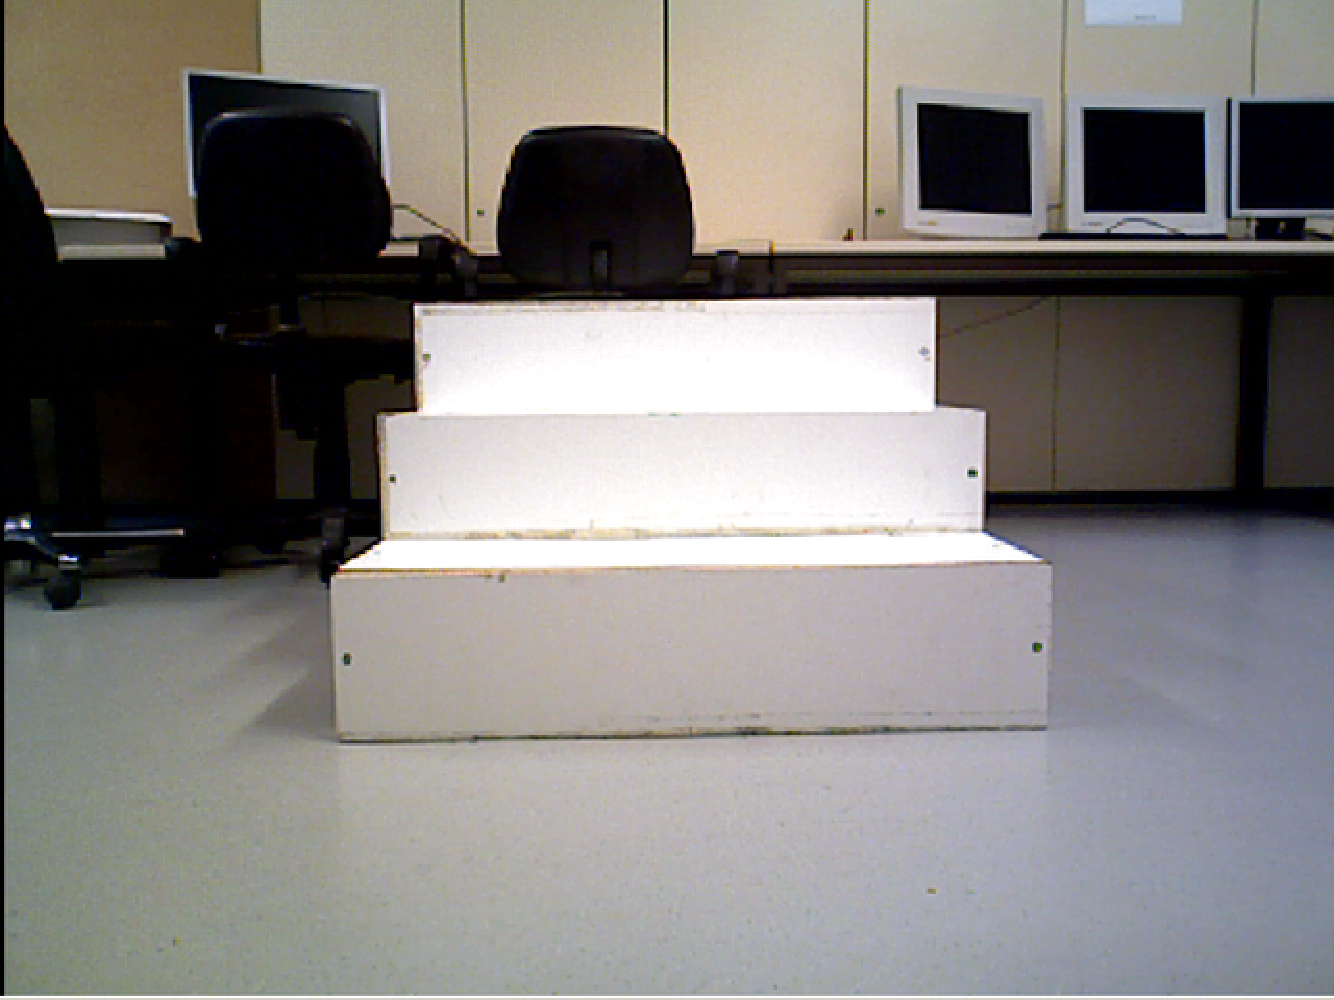
\includegraphics[scale=0.16]{images/canny00.pdf}\newline
			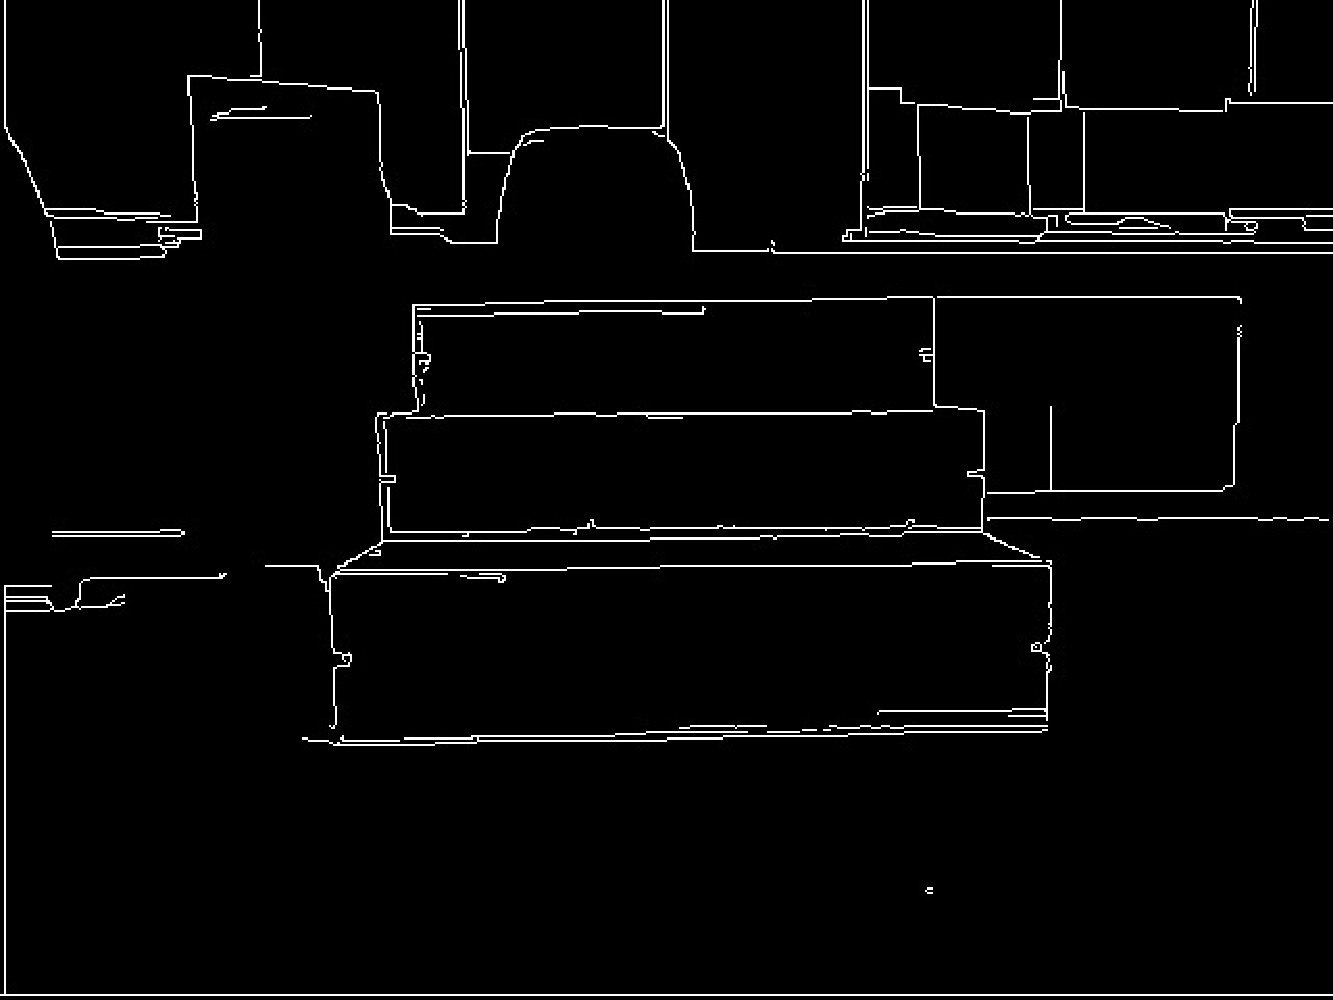
\includegraphics[scale=0.16]{images/canny02.pdf}
		\column{0.25\textwidth}
			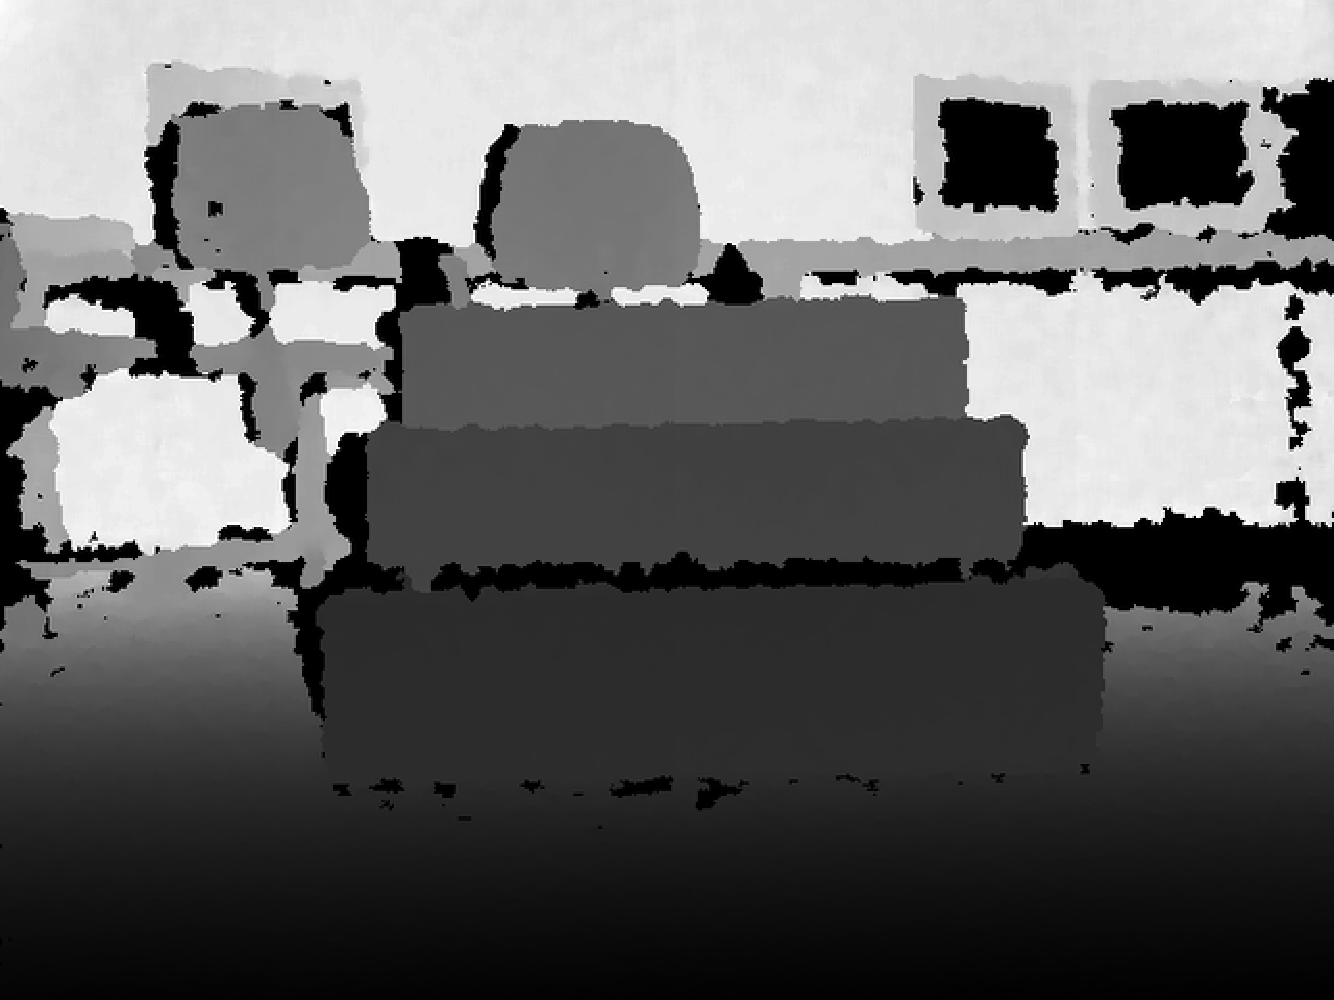
\includegraphics[scale=0.16]{images/canny01.pdf}\newline
			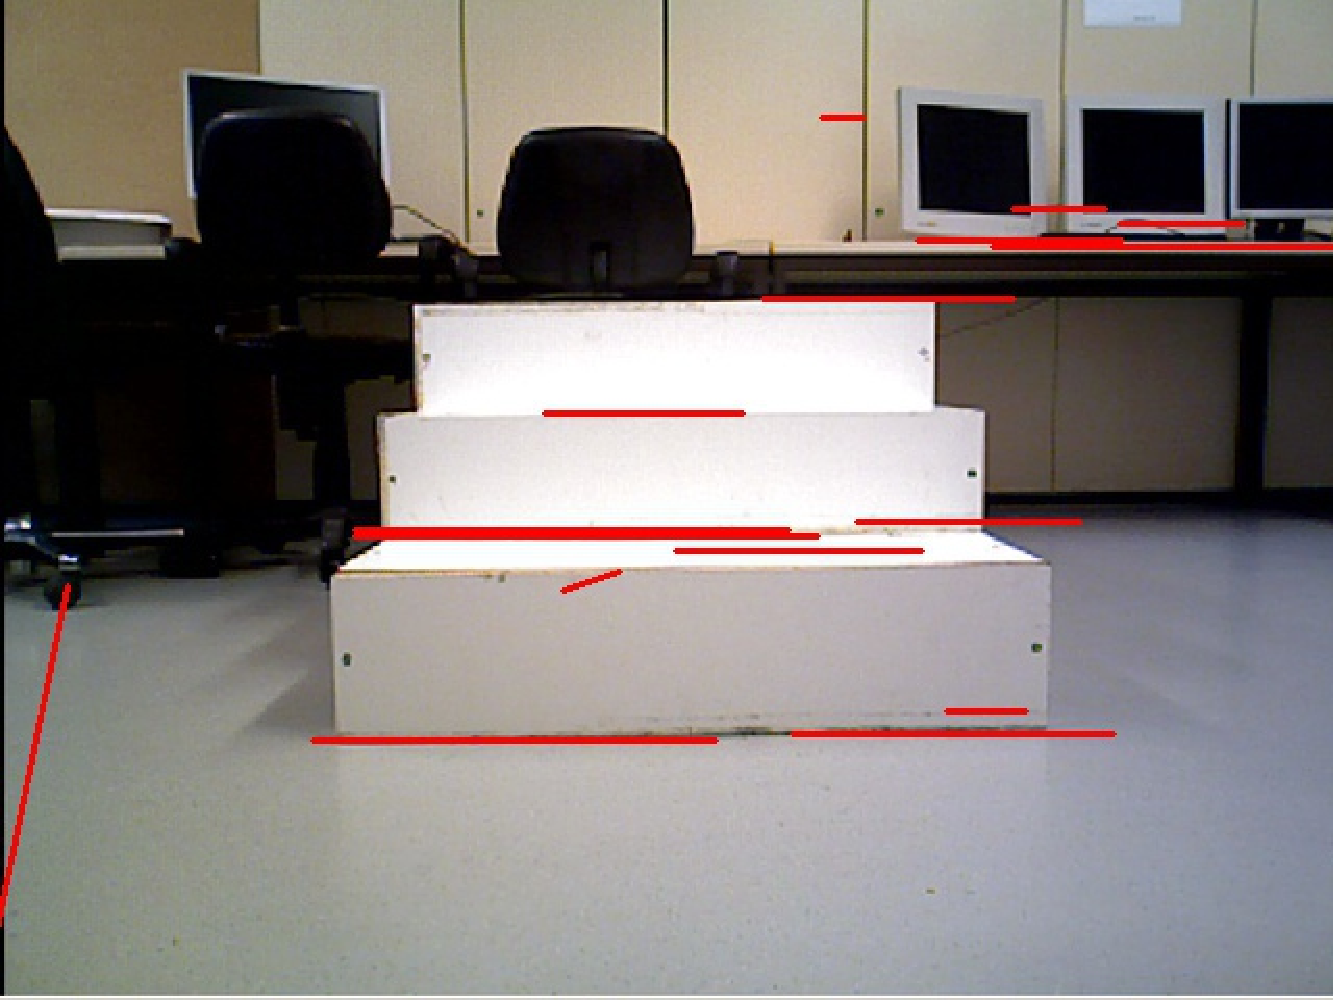
\includegraphics[scale=0.16]{images/canny03.pdf}
	\end{columns}
\end{frame}


\subsection{Ansatz 2: Erkennen von Treppen mittels vertikaler Flächen}
\begin{frame}{Ansatz 2: Erkennen von Treppen mittels vertikaler Flächen}
	\begin{itemize}
		\item Eingabe: zwei-dimensionale Punktwolke
		\item Verwendung des RANSAC-Algorithmus zur Ermittlung von Flächen (dazu gleich mehr)
		\item \dots
	\end{itemize}
\end{frame}

\begin{frame}{RANSAC-Algorithmus}
	\begin{itemize}
		\item Blabla
		\item Linien und Flächen
		\item Blabla
	\end{itemize}
\end{frame}



\section{Implementierung}

\begin{frame}{Implementierung}
	\begin{itemize}
		\item ROS Node
		\item C++, PCL
		\item Einführen eines Ebenen-Formats
		\item Import-/Export-Funktion
		\item \dots
	\end{itemize}
\end{frame}

\begin{frame}{Implementierung im Detail}
	\begin{enumerate}
		\item Empfangen und Downsamplen der Punktwolke
		\item Aktivitätsdiagramm
		\item \dots
	\end{enumerate}
\end{frame}

\begin{frame}{Implementierung im Detail}
	\begin{itemize}
		\item Eingabe: Punktwolke
	\end{itemize}
	\begin{center}
		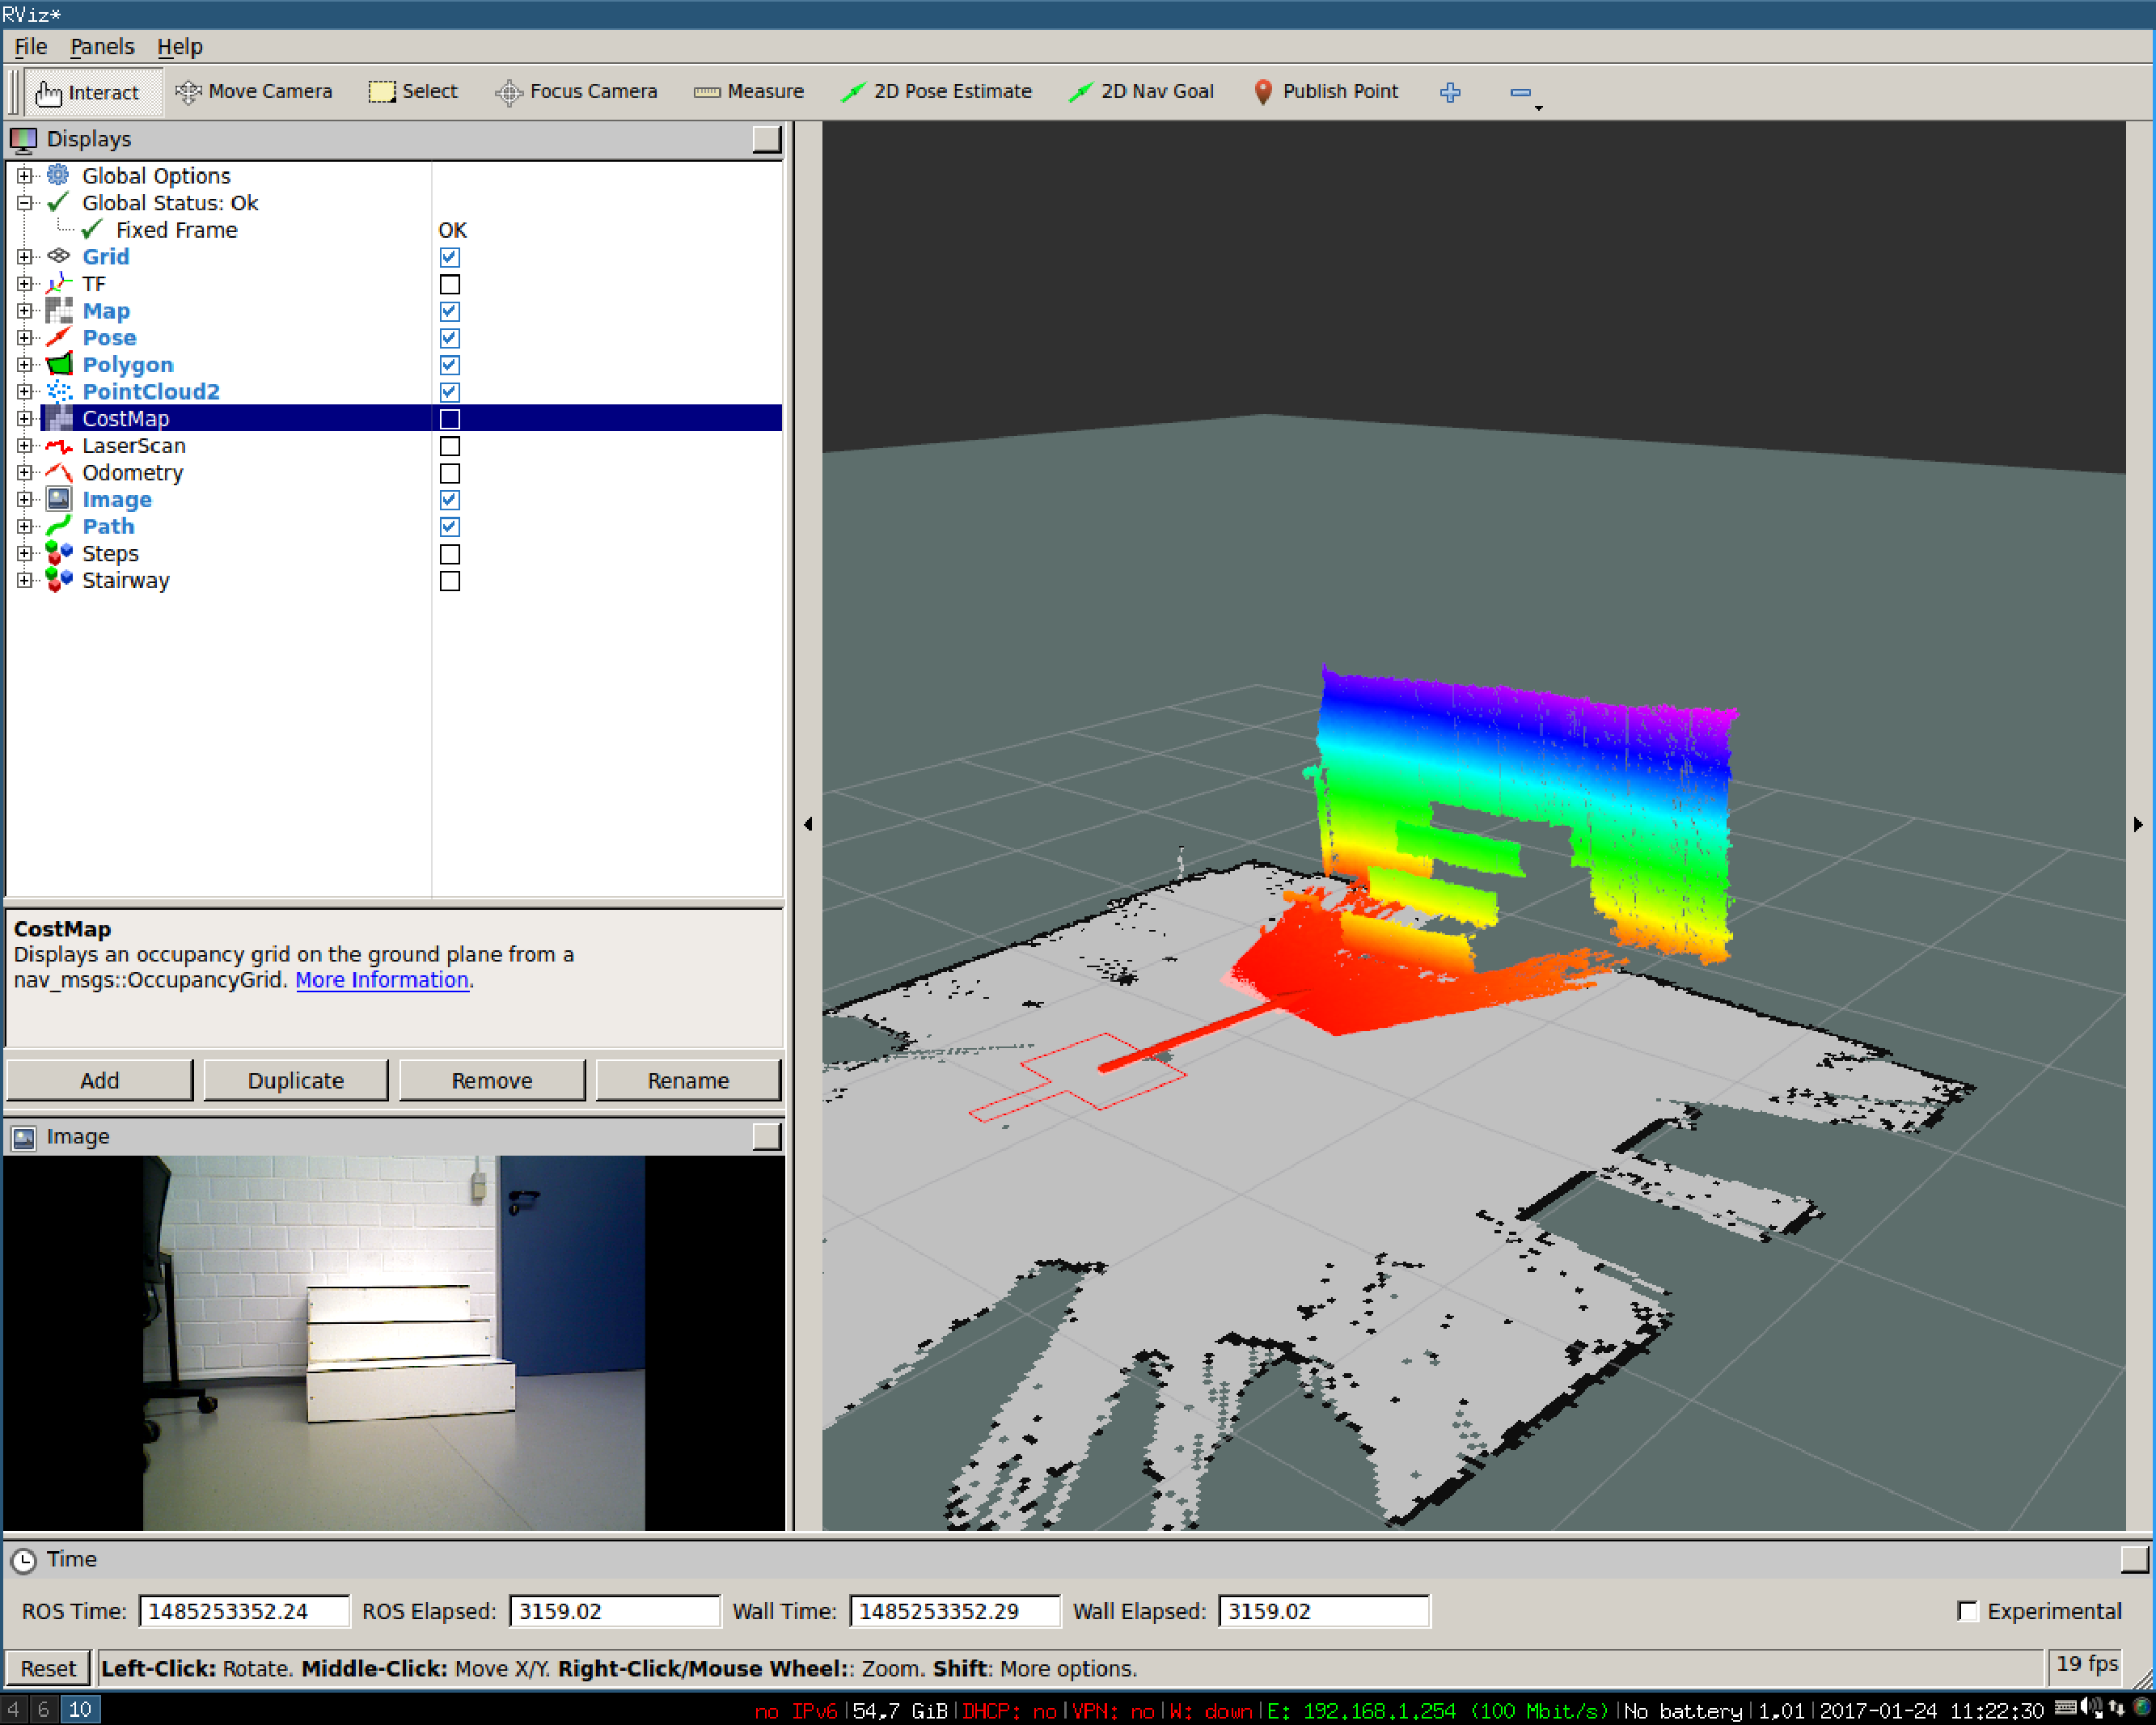
\includegraphics[scale=0.16]{images/ransac00.pdf}
	\end{center}
\end{frame}

\begin{frame}{Implementierung im Detail}
	\begin{itemize}
		\item Nach Anwendung von \texttt{RANSAC}: Erkennen von senkrechten Flächen
	\end{itemize}
	\begin{center}
		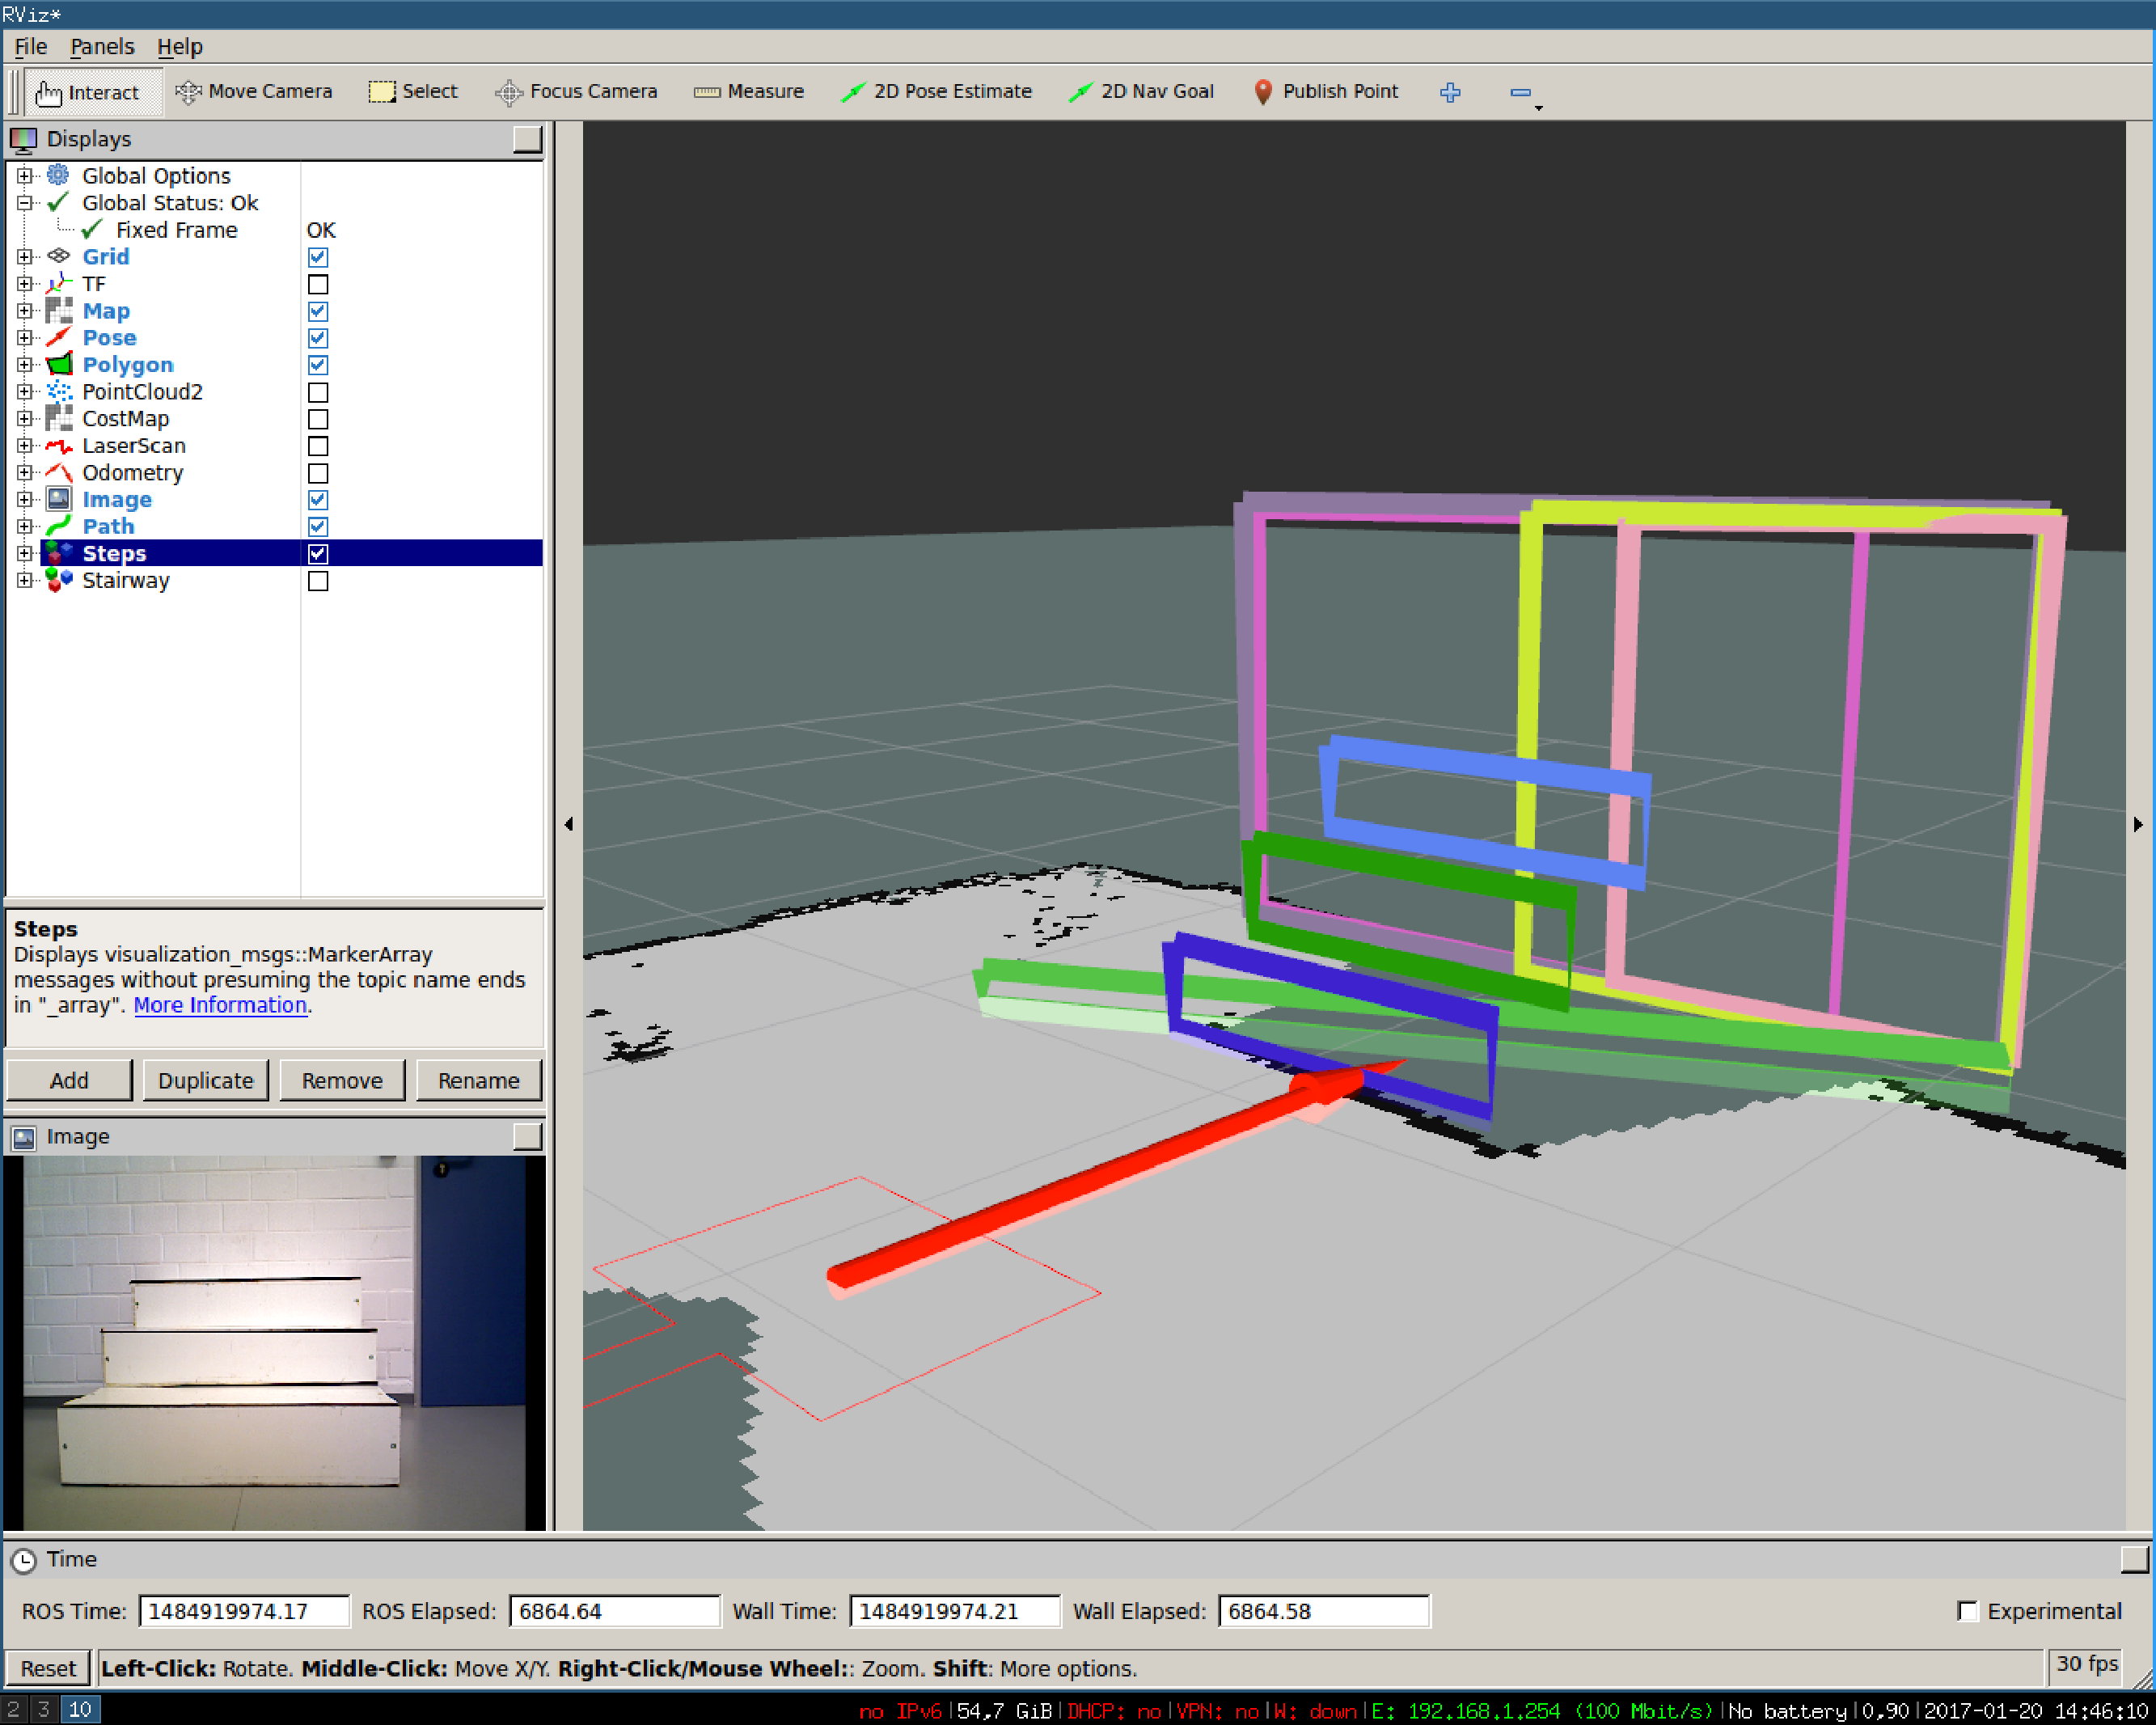
\includegraphics[scale=0.16]{images/ransac01.pdf}
	\end{center}
\end{frame}

\begin{frame}{Implementierung im Detail}
	\begin{itemize}
		\item Höhenfilter
	\end{itemize}
	\begin{center}
		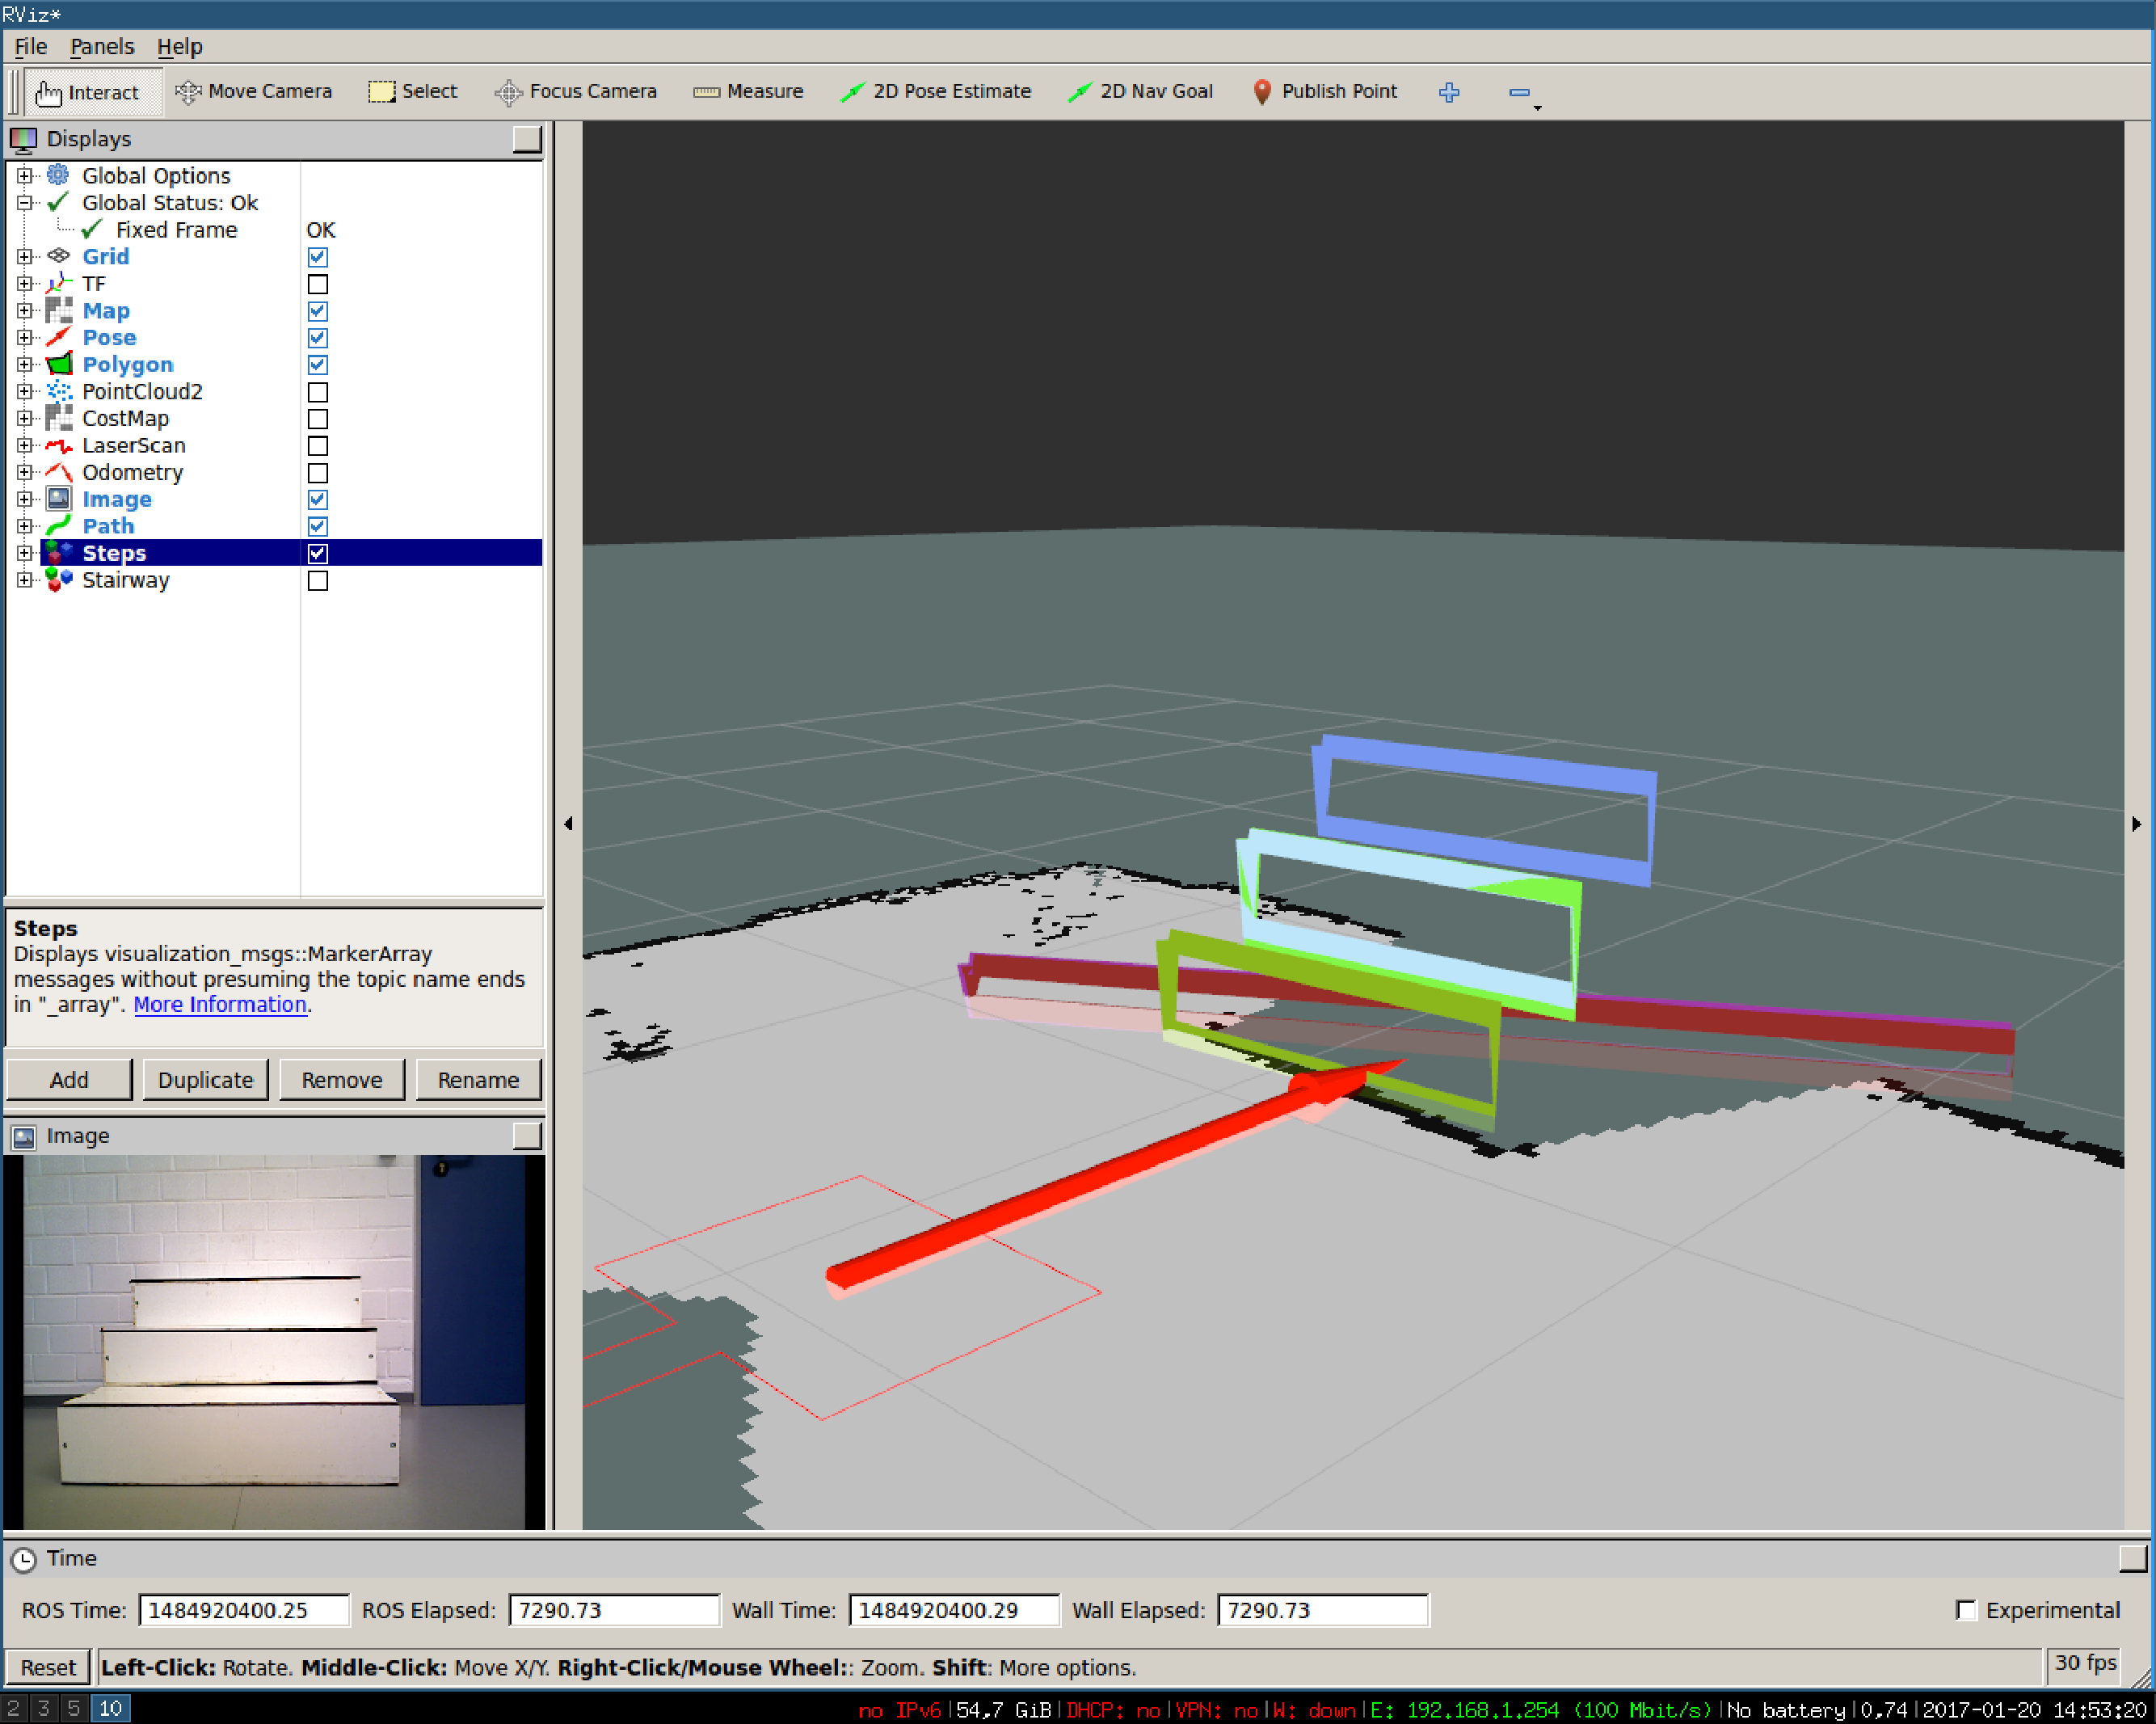
\includegraphics[scale=0.16]{images/ransac02.pdf}
	\end{center}
\end{frame}

\begin{frame}{Implementierung im Detail}
	\begin{itemize}
		\item Treppenbauen
	\end{itemize}
	\begin{center}
		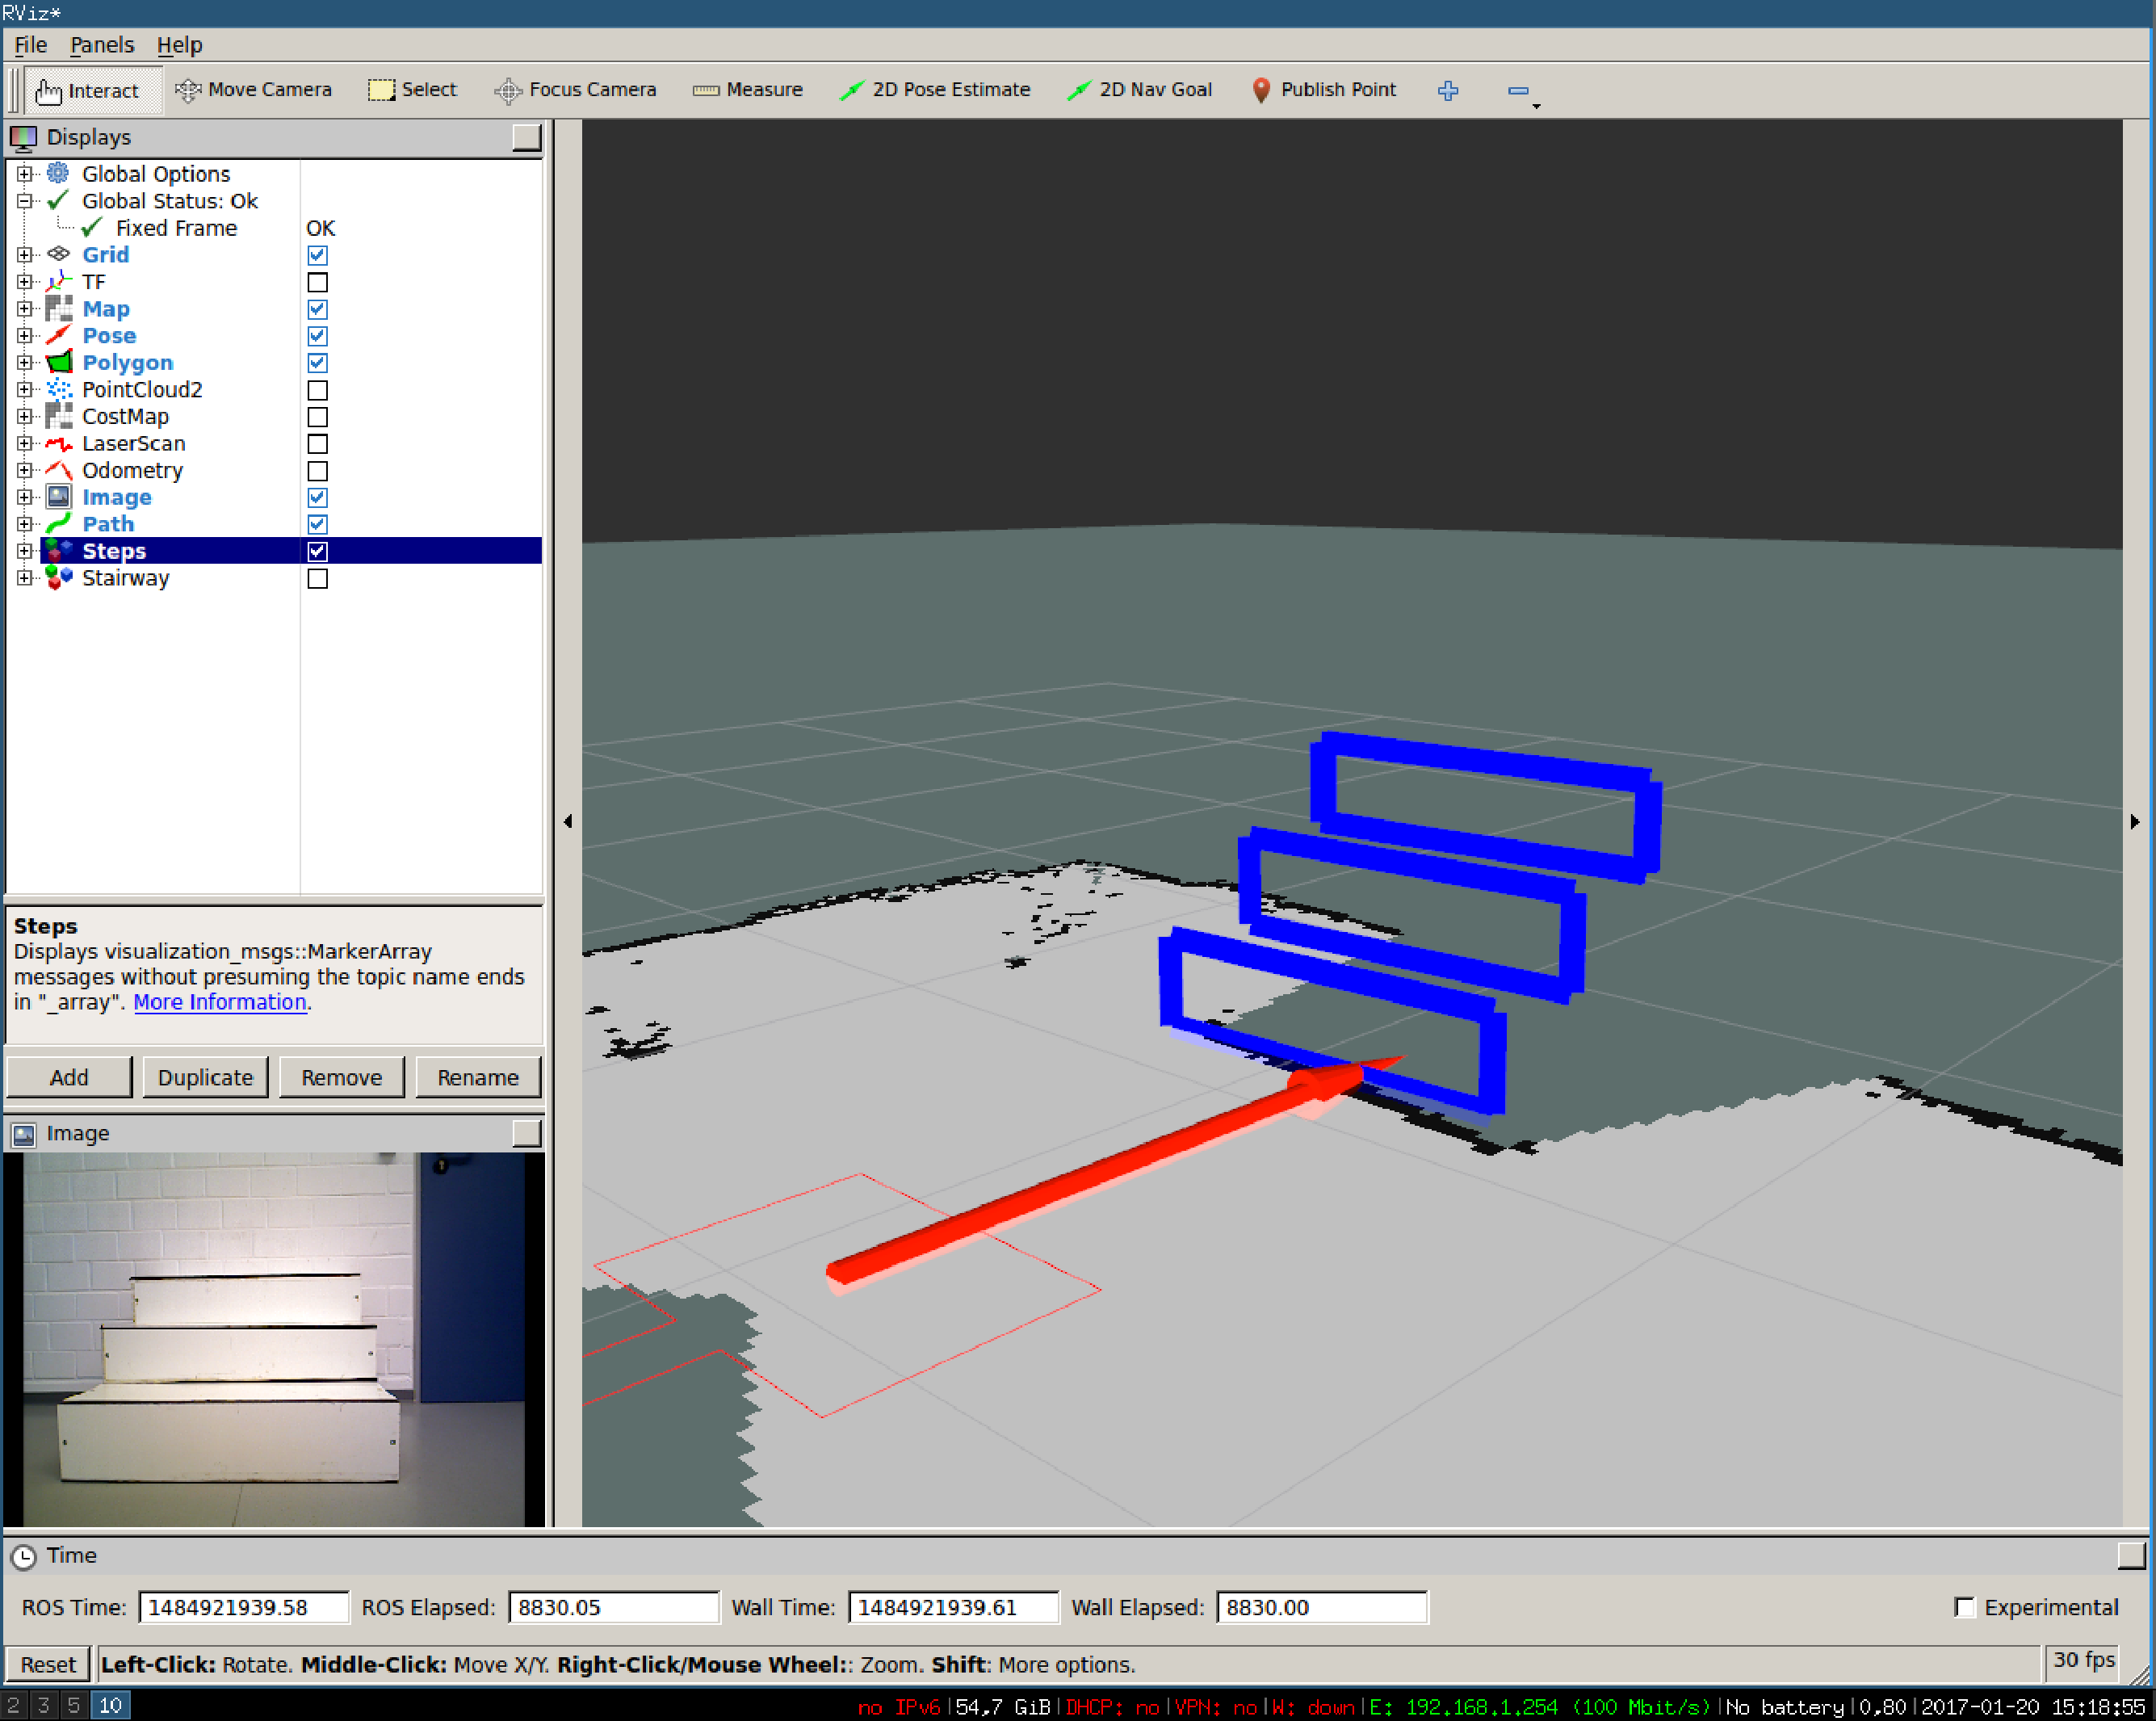
\includegraphics[scale=0.16]{images/ransac03.pdf}
	\end{center}
\end{frame}

\begin{frame}{Speicherformat für Import/Export}
	\begin{itemize}
		\item \texttt{rosservice call export\_stairways \~stairs.yaml}
	\end{itemize}

\end{frame}



\section{Bewertung des Ergebnisses}

\begin{frame}{Bewertung des Ergebnisses}
Was wurde erreicht?
\end{frame}

\begin{frame}{Probleme/Schwächen}
Probleme/Schwächen
\end{frame}

\begin{frame}{Ausblick}
Ausblick
\end{frame}





%\appendix
%\beginbackup

%\begin{frame}[allowframebreaks]{References}
%\printbibliography
%\end{frame}

%\backupend

\end{document}
